% 英文で執筆する場合はクラスファイルへのオプションを[T,E]としてください.
% If you want to write your paper in English, pass to [T,E] options to document class.
\documentclass[T,J]{fose} % 「コンピュータソフトウェア」用のクラスファイルは compsoft です.
\taikai{2024} % 固定です.出版委員長が毎年変更してAuthor Kitを配布してください.

\usepackage [dvipdfmx] {graphicx}
\usepackage{xcolor} % 色を扱うためのパッケージ
% ユーザが定義したマクロなどはここに置く.ただし学会誌のスタイルの
% 再定義は原則として避けること.

% 以下は説明のために使用したパッケージであるため,削除可能.
\usepackage{listings}
\usepackage{tabularx}
\usepackage{fancyvrb}
\usepackage{xurl}
\usepackage{cite}
\usepackage[dvipdfmx]{graphicx}
\usepackage{latexsym}
\usepackage[T1]{fontenc}
\usepackage{lmodern}
\usepackage{textcomp}
\usepackage{latexsym}
\usepackage{url}
\usepackage{multirow}
% 以下のマクロはサンプルファイル作成用のマクロです.不要であれば削除してください.
\newcommand{\foseclassfile}{fose.cls}
\newcommand{\fosestylefile}{fose.sty}
\newcommand{\todo}[1]{\colorbox{yellow}{{\bf TODO}:}{\color{red} {\textbf{[#1]}}}}
\newcommand{\change}[1]{\colorbox{green}{{\bf CHANGE}:}{\color{red} {\textbf{[#1]}}}}

\begin{document}

% 論文のタイトル 
\title{JavaScriptライブラリの後方互換性の損失によるクライアントへの影響範囲の特定}
% 以下の \etitle(と\@etitle)はFOSE論文フォーマット独自のマクロです.
% FOSEに投稿した論文を発展させてコンピュータソフトウェアに投稿される場合はコメントアウトしてください.
% \setetitleは奇数ページのヘッダに表示する文字列(\etitle)を設定するためのマクロです.
% タイトルが2行に渡る場合は "\\" を 使用することで任意の位置で改行をすることができます.
\setetitle{Identification of Clients due to Loss of JavaScript Library Backward Compatibility}
%\setetitle{Long Long Long Long Long Long \\ Long Long Long Long Long \\ Long Long Long Long Long Long Long Long Long Long Long Long Paper Title}

% タイトル,著者などが複数行にわたり,論文冒頭の著者名が日本語アブストと重複して描画された場合に以下のコメントアウトを外してください.
%\longtitle

% 著者
% 和文論文の場合,姓と名の間には半角スペースを入れ,
% 複数の著者の間は全角スペースで区切る
%
\author{飯田 智輝 伊原 彰紀
%
% ここにタイトル英訳 (英文の場合は和訳) を書く.
% 英語タイトルは論文1ページ目左下,著者らの名前・所属一覧の一番上に表示される
%
% 上記\setetitle中で改行した場合は "\etitle" を削除し,改行(\\)を入れていないタイトルを記載してください.
% \ejtitleは1ページ目左下に挿入されるタイトルとして使用されます.
% また,"\etitle"はFOSE論文フォーマット独自のマクロです.
\ejtitle{\etitle}
%
% ここに著者英文表記 および
% 所属 (和文および英文) を書く.
% 複数著者の所属はまとめてよい
% 複数著者の所属は以下のようにまとめてよい.
\shozoku{Tomoki Iida, Akinori Ihara}{和歌山大学}
{Wakayama University}
}
%
% 和文アブストラクト

% In English paper, content of Jabstract will be ignored. 
\Jabstract{%
ソフトウェア開発では,開発効率を上げるために特定の機能がまとめられたライブラリを利用する.ライブラリ開発者がライブラリの品質を維持するために機能追加や修正などを行いバージョン更新する中で,既存機能の変更や削除によって後方互換性を損失することがある.後方互換性の損失はライブラリを利用するクライアントソフトウェアの振る舞いの阻害につながるが,ライブラリ開発者がクライアントソフトウェアを実行することなく影響範囲を特定することは容易ではない.本研究では,ライブラリ更新後にクライアントテストが失敗となったクライアントから依存ライブラリに関わるソースコード断片を抽出し,後方互換性の損失の原因となるソースコード断片からライブラリと関数の呼び出し文の記述パターンを作成する.作成した記述パターンをもとにテストが成功しているクライアントを分析することで,実際には影響を受けているクライアントを特定する.
}
%
% 英文アブストラクト(本サンプルの原論文にはなし)
% \Eabstract{
% This document has been prepared as a sample for FOSE(Foundation of Software Engineering) based on the Author Kit for rePiT and FOSE2022.
% The author kit for rePiT was originally based on author kit of JSSST Computer Software.
% The detail changes are written in Sec.\ref{sec:PaperStyle}
% }
%
\maketitle \thispagestyle {empty}

%%%%%%%%%%%%%%%%%%%%%%%%%%%%%
\section{はじめに}
%%%%%%%%%%%%%%%%%%%%%%%%%%%%%

ソフトウェア開発を効率的に進めるために機能が使いやすい形にまとめられたライブラリが広く公開されている.開発者はライブラリの利用により,開発者自身が同じ機能を再実装する必要がなくなるため開発効率が向上する\cite{konstantopoulos2009best}\cite{Moser1996effect}.ソフトウェアが新機能追加,バグ修正によって頻繁にソースコードを更新されるように,ライブラリも例外ではない\cite{raemaekers2012measuring}.ライブラリの更新には,脆弱性の修正などライブラリを利用するクライアントソフトウェア(以降,クライア
ント)にとって重要な変更が含まれることがあり,ライブラリのバージョン更新は,ライブラリを再利用するクライアントが依存ライブラリの更新を余儀なくされることも多い.

ライブラリのバージョン更新はソフトウェアの品質維持のために重要であるが,ライブラリ更新に機能削除や仕様変更といったクライアントに影響を与える変更が含まれる場合,更新前後でライブラリのソースコードに不整合が生じ,クライアントが実行時エラーになることがある.このように,更新後の依存ライブラリがクライアントに影響を与えることを後方互換性を損失するという.通常は,後方互換性を損失するバージョンをリリースする場合,バージョン名で後方互換性を損失する変更を含むことが周知できるようメジャーバージョンとしてリリースする.しかし,バージョン名の付与はライブラリ開発者が手動で行うため,後方互換性を損失しているにもかかわらず誤ってマイナーバージョンとしてリリースすることもあり,当該変更に関して機能の動作変更内容が文書化されていないことがある\cite{mostafa2017experience}.

Mujahidらは,後方互換性を損失するJavaScriptライブラリバージョンを特定するために,ライブラリ更新前後のクライアントテストを確認する実験を行っている\cite{mujahid}.当該研究は,クライアントテストの成否をもとに影響を受けたクライアントを把握しているが,クライアントテストが不十分な場合に後方互換性の損失の影響を受けていることを検出できない.事前分析としてuuidの2つのバージョンを調査した結果,後方互換性を損失する多くのライブラリは,ライブラリの呼び出し文と関数の呼び出し文を変更しており,本研究ではライブラリと関数の呼び出し文の記法に着目する.ただし,本研究の事前分析において,後方互換性を損失する場合にライブラリの呼び出し文と対応する関数の呼び出し文が多様であることを明らかにした.本研究では,多様なライブラリと関数の呼び出し文から記述パターンを生成し,テストに成功したクライアントの中でライブラリの後方互換性の損失の影響を受けるクライアントを特定する.特に,クライアントのテストから発見できる構文的な互換性と振る舞い的な互換性の両方を分析対象とする.

以降,本論文では,\ref{chap:intro}章で後方互換性の損失と従来研究について述べる.\ref{sec:method}章で後方互換性が損失するライブラリの呼び出し文,および関数呼び出し文の記述パターンの生成方法を述べる.\ref{chap:case_study}章でケーススタディのためのデータセットおよび分析結果を述べ,\ref{sec:conclusion}章でまとめる.



%----------------------
\begin{figure*}[ht]
\centerline{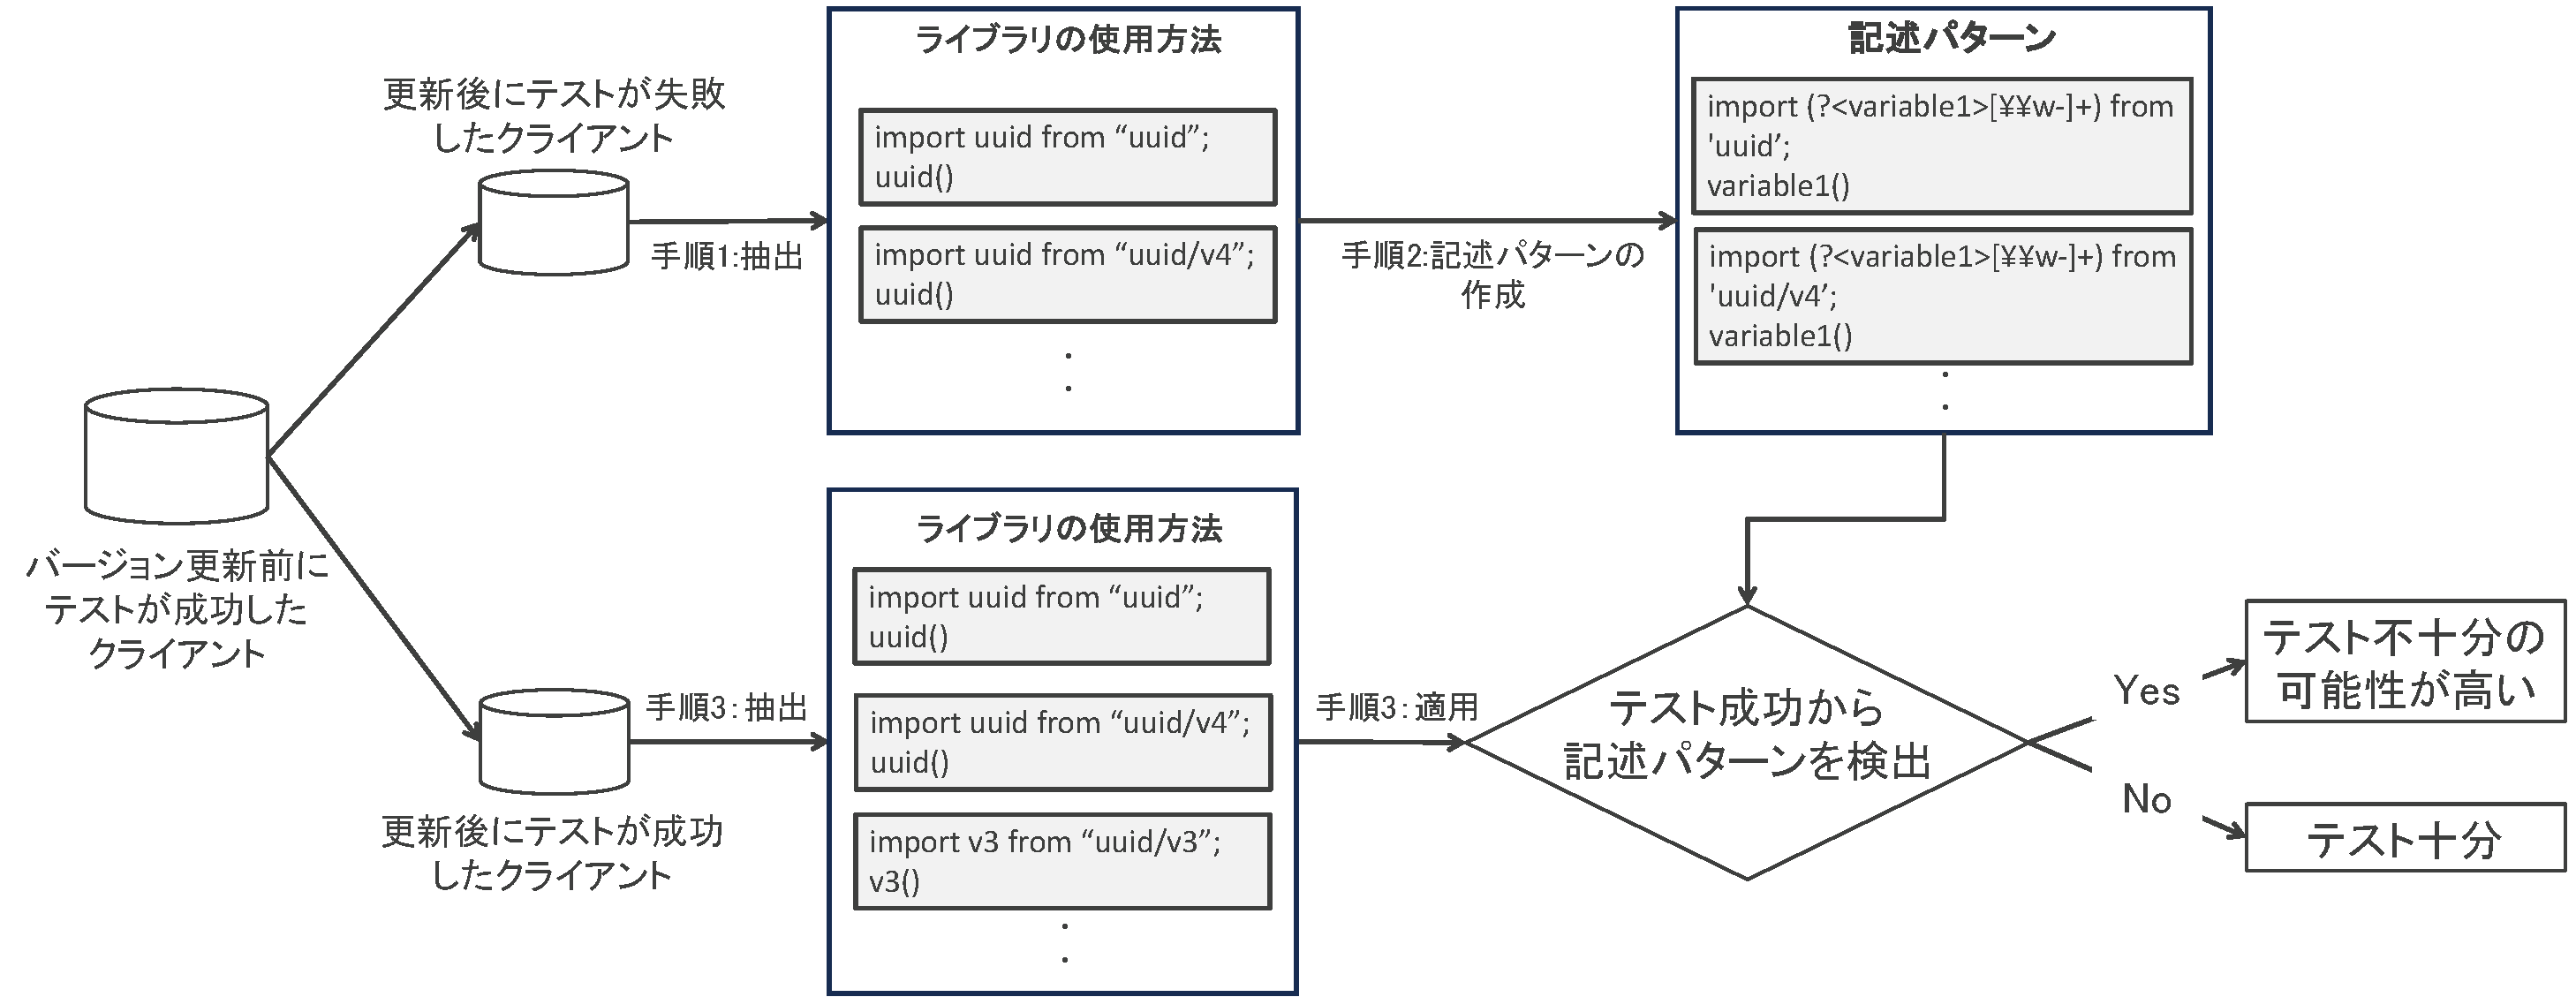
\includegraphics[width=1.0\linewidth]{Iida_fig/Fose_method.pdf}}
\caption{後方互換性の損失によるクライアントの特定手法の概略図}
\label{fig:method-overview}
\end{figure*}
%----------------------


%%%%%%%%%%%%%%%%%%%%%%%%%%%%%
\section{後方互換性の損失}\label{chap:intro}
%%%%%%%%%%%%%%%%%%%%%%%%%%%%%

\subsection{後方互換性の損失の課題}
ライブラリを利用することで効率的にソフトウェアを実装できるが,使用するライブラリバージョンの更新に後方互換性の損失が含まれるとクライアントが実行時エラーを引き起こすことがある.ライブラリバージョンに後方互換性の損失を含む場合,クライアントはライブラリのバージョンをダウングレードするか,後方互換性の損失の影響を受けない書き方に書き換えるか,または影響を受ける機能の使用を停止することになる.後方互換性の損失を含むライブラリをリリースする場合,ライブラリ開発者は影響を受けない書き方を公開することもあるが,既存機能の変更に関する文書化がされていないことが多く,開発者にとってライブラリの更新判断や修正にかけるコストが増加している\cite{mostafa2017experience}.



\subsection{従来研究}
ライブラリバージョンの更新における後方互換性の損失の有無を判定する手法としてテストを用いる手法が提案されている\cite{mujahid}\cite{matsuda}.Mujahidらは,ライブラリの後方互換性の損失の有無を判定するために,該当ライブラリに依存するクライアントテストを用いた手法を提案している\cite{mujahid}.当該手法は,ライブラリバージョン更新前後でクライアントテストを実行し,成功していたテストが依存ライブラリの更新後に失敗すれば後方互換性の損失と判定する.また,松田らは,ライブラリの機能の変更に伴うライブラリのテスト変更の有無から後方互換性の損失の有無を判定する手法を提案しており,クライアントテストの実行結果をもとにした後方互換性の損失有無の判定を評価に利用している\cite{matsuda}.M{\o}llerらは,後方互換性の損失への対処を支援するために後方互換性の損失の影響を受けるクライアントのプログラムの場所を検出する手法を提案している\cite{10.1145/3428255}.この手法では,後方互換性の損失の影響を受ける記述パターン集を手作業で作成し,パターン集をもとにクライアントのソースコードを静的に解析することで影響を受ける場所を検出している.ただし,テストが成功しているクライアントの中で実際には後方互換性の損失の影響を受ける範囲は分析していない.


\subsection{動機}
ライブラリ開発者は,ライブラリの変更によってクライアントの振る舞いに影響を与えるライブラリの呼び出し方を確認することで,後方互換性の損失によるクライアントへの影響範囲を特定できる.しかし,ライブラリ更新のたびにクライアントのソースコードから使用方法を確認することはコストが膨大になるため現実的でない.


本研究では,依存ライブラリバージョンの更新に伴って後方互換性の損失の影響を受けたクライアントは,ライブラリが周知するライブラリの呼び出し方,関数の呼び出し方をしていたのか調査する.JavaScriptライブラリであるuuidで後方互換性の損失を含む2種類のバージョン更新(uuid@7.0.3...8.0.0-beta.0,uuid@3.4.0...7.0.0-beta.0\footnote{本論文ではバージョン更新前後のバージョン名を``更新前バージョン名...更新後バージョン名''と記す.})のいずれかを実施し,テストを失敗したクライアントにおけるライブラリの使用方法を目視調査した.バージョン8.0.0-beta.0および7.0.0-beta.0の後方互換性の損失に関係する呼び出し方はWebサイトに公開されている\footnote{https://github.com/uuidjs/uuid/blob/v7.0.0/\\CHANGELOG.md}\footnote{https://github.com/uuidjs/uuid/blob/v8.0.0/\\CHANGELOG.md}.ここで文書化されているのは,実際に失敗した原因の一部である.例えば,7.0.0-beta.0において「import * as uuid from 'uuid', uuid();」の使い方は言及されていないがv7.0.0では使用できない呼び出し文である.本研究では,このようなライブラリ更新後にクライアントテストが失敗したクライアントから依存ライブラリに関わるソースコード断片を抽出し,後方互換性の損失の原因となるソースコード断片からライブラリと関数の呼び出し文の記述パターンを作成することで,後方互換性の損失の影響を受けるクライアントを特定する.特に,構文的な互換性と振る舞い的な互換性の両方を含むクライアントテストの失敗を引き起こす後方互換性の損失を分析対象とする.



%%%%%%%%%%%%%%%%%%%%%%%%%%%%%
\section{後方互換性の損失によるクライアントの特定手法}\label{sec:method}
%%%%%%%%%%%%%%%%%%%%%%%%%%%%%

本章では,依存ライブラリの更新に伴いテストが失敗したクライアントから後方互換性の損失の影響を受ける呼び出し文,および関数呼び出し文の記述パターンを生成する手法を述べる.本研究でクライアントテストは,ライブラリを使用するクライアントの開発者が単体テストや結合テストのために準備したテストケースを指し,ライブラリバージョンの更新前後でクライアントテストの結果が成功から失敗に変わったものを「テストが失敗」,テスト失敗以外のクライアントを「テストが成功」と定義する.図\ref{fig:method-overview}に後方互換性の損失によるクライアントの特定手法の概略図を示し,各手順の説明を述べる.



\noindent\textbf{手順1.テストが失敗したクライアントからライブラリの呼び出し文,関数呼び出し文を抽出}

クライアントのJavaScriptまたはTypeScriptで記述されたソースコードファイルを抽象構文木に変換し,ライブラリの呼び出し文(\texttt{import}文,\texttt{require}文),およびライブラリの関数呼び出し文を抽出する.

\noindent\textbf{手順2.ライブラリ呼び出し文,関数呼び出し文の記述パターンの生成}

ライブラリ呼び出し文,関数呼び出し文の変数名や関数名を抽象化したのち,正規表現として記述パターンを生成する.具体的には,図\ref{fig:method-overview}における変換は,表\ref{table:abstractionsample}のようにして行われる.

%-----------------------
\begin{table}[t]
\caption{記述パターンの作成例}
\label{table:abstractionsample}
\scalebox{0.65}{
\begin{tabular}{l|l}
\hline
    変換前 & 変換後 \\ \hline \hline
    \begin{tabular}[c]{@{}l@{}}import uuid from ``uuid''\\ uuid();\end{tabular} & \begin{tabular}[c]{@{}l@{}}import (?\textless{}variable1\textgreater{}{[}w-{]}+) from `uuid';\\ variable1()\end{tabular} \\ \hline
    \begin{tabular}[c]{@{}l@{}}import v4 from ``uuid/v4'';\\ v4();\end{tabular} & \begin{tabular}[c]{@{}l@{}}import (?\textless{}variable1\textgreater{}{[}w-{]}+) from `uuid';\\ variable1()\end{tabular} \\ \hline
    \begin{tabular}[c]{@{}l@{}}import uuid from ``uuid'';\\ uuid.v4()\end{tabular} & \begin{tabular}[c]{@{}l@{}}import (?\textless{}variable1\textgreater{}{[}w-{]}+) from `uuid';\\ variable1.v4()
    \end{tabular} \\ \hline
\end{tabular}
}
\end{table}
%-----------------------


ライブラリ呼び出し文,関数呼び出し文において,各クライアントが命名した変数名,関数名は図\ref{fig:method-overview}の\texttt{variable}のように抽象化して表現する.抽象化後にライブラリの呼び出し文とライブラリの関数呼び出し文を紐づけるため,抽象化した名前に図\ref{fig:method-overview}の\texttt{variable1}のようなIDを付与し,1つのクライアントで共通する変数名を紐づける.また,改行のような特殊文字や記述パターンの前後の空白は,必要ないため削除する.「mockImplementation」のようなモック関数を含むクライアントのライブラリ使用部分の抽象化において特殊な名付けを考慮することは困難なため今後の課題とする.生成した記述パターンにおいて包含関係のあるパターン対が存在する場合には,手動でパターン集約を行う.パターン集約では,広く検出できるパターンを残すためパターンを集約することによる検出誤りのリスクはない.また,パターン集約の作業は記述パターンを比較し,包含関係にあるかどうかを確認するだけのため時間はかかるものの,複雑な判断は必要としない.そのため,集約の際に誤りが起こる可能性は低い.



ライブラリ関数の引数がクライアントで定義されている場合には,引数の中身は保持せず引数の数のみを確認するように記述パターンを変換する.本研究において各クライアントが命名した変数名,関数名の影響を抽象化によって取り除いているが,引数が変数としてまとめられている場合には引数の数を判断できない問題がある.しかし,ライブラリ開発者は,誤った記述パターンを提示された際に誤りの有無を判別できると考えられるため,
検出する再現率が向上するように抽象度の高い記述パターンを生成する.フィルタリング,抽出,抽象化を含む処理をテストに失敗したクライアントのリポジトリごとに行い,クライアントごとにまとめることで記述パターンを作成する.ただし,ライブラリ呼び出し単体しか記述パターンを抽出できなかったクライアントは,特殊な呼び出し文である可能性が高いためパターンを生成しない.


\noindent\textbf{手順3.クライアントテストが成功する中で後方互換性の損失による影響を受けるクライアントの検出}

後方互換性の損失の影響を受けたクライアントのライブラリ呼び出し文から生成した記述パターンを用いて,テストが成功しているクライアントの中で後方互換性の損失の影響を受けたクライアントと同じ呼び出し文を使用しているクライアントを検出する.具体的には,クライアントの\texttt{import}や\texttt{require}から始まるライブラリの呼び出し文を検出する.続いて関数呼び出し文もライブラリ呼び出し文と同様に,テストが成功しているクライアントの中に後方互換性の損失の影響を受けたクライアントと同じ関数呼び出し文を使用しているクライアントを検出する.


%---------------------

\begin{table}[t]
    \caption{分析対象としたライブラリ}
    \label{table:dataset}
    \centering
    \scalebox{0.7}{
        \begin{tabular}{p{4cm}|p{1.5cm}|p{1.5cm}|p{1.5cm}}
        \hline
        ライブラリ名@\par 旧バージョン{...}新バージョン & 更新前の\par テスト成功 & 更新後の\par テスト失敗 & 更新後の\par テスト成功 \\
        \hline
        uuid@7.0.3…8.0.0-beta.0 & 433 & 118 & 315 \\
        uuid@3.4.0…7.0.0-beta.0 & 492 & 57 & 435 \\
        globby@8.0.0…8.0.1 & 128 & 42 & 86 \\
        globby@6.1.0…7.0.0 & 137 & 27 & 110 \\
        meow@3.6.0...4.0.0 & 153 & 26 & 127 \\
        pump@1.0.3...2.0.0 & 112 & 19 & 83 \\
        globby@7.1.1…8.0.0 & 143 & 17 & 126 \\
        vinyl@1.2.0…2.0.0 & 69 & 11 & 58 \\
        \hline
        \end{tabular}
    }
\end{table}
%---------------------
%%%%%%%%%%%%%%%%%%%%%%%%%%%%%
\section{ケーススタディ}\label{chap:case_study}
%%%%%%%%%%%%%%%%%%%%%%%%%%%%%
\begin{table*}[t]
     \caption{パターンを取得できたクライアント数}
     \label{table:all client_pattern}
    \centering
     \scalebox{0.60}{
         \begin{tabular}{l|r|r|r|r|r}
         \hline
         \begin{tabular}{c} ライブラリ名@\\旧バージョン{...}\\新バージョン \end{tabular}
         & \begin{tabular}{c} 更新後にテストを\\失敗した\\クライアント数 \end{tabular}
         & \begin{tabular}{c} 記述パターンを\\取得できた\\クライアント数 \end{tabular}
         & \begin{tabular}{c} 記述パターンを\\取得できなかった\\クライアント数 \end{tabular}
         & 集約パターン数
         & \begin{tabular}{c} 検出時に使用した\\記述パターン数 \end{tabular}
         \\ \hline
         uuid@7.0.3…8.0.0-beta.0 & 118 & 102 & 16 & 16 & 5\\
         uuid@3.4.0…7.0.0-beta.0 & 57 & 53 & 4 & 16 & 7\\
         globby@8.0.0…8.0.1 & 42 & 41 & 1 & 21 & 9\\
         globby@6.1.0…7.0.0 & 27 & 24 & 3 & 13 & 7\\
         meow@3.6.0...4.0.0  & 26 & 11 & 15 & 4 & 2\\
         pump@1.0.3...2.0.0 & 19 & 17 & 2 & 3 & 2\\
         globby@7.1.1…8.0.0 & 17 & 15 & 2 & 10 & 9\\
         vinyl@1.2.0…2.0.0  & 11 & 10 & 1 & 3 & 1\\
         \hline
         \end{tabular}
         }
\end{table*}

\begin{table*}[t]
    \caption{uuid@7.0.3…8.0.0-beta.0の記述パターン}
    \label{table:uuidclient_pattern}
    \centering
    \scalebox{0.6}{
        \begin{tabular}{c|l|r|r}
        \hline
        \multicolumn{1}{c|}{ID} & \multicolumn{1}{c|}{記述パターン}& \multicolumn{1}{c|}{統合数(重複数)} & \multicolumn{1}{c}{クライアントへの該当数} \\ \hline\hline
        1& \begin{tabular}[c]{@{}l@{}}"(?\textless{}variable1\textgreater{}{[}\textbackslash{}\textbackslash{}w-{]}+) = require('uuid/v4')" \\ "variable1()"\end{tabular}  & 54 & 25 \\ \hline
        2 & \begin{tabular}[c]{@{}l@{}}"import (?\textless{}variable1\textgreater{}{[}\textbackslash{}\textbackslash{}w-{]}+) from 'uuid/v4'"\\ "variable1()"\end{tabular} & 13 & 4  \\ \hline
        3 & \begin{tabular}[c]{@{}l@{}}"const (?\textless{}variable1\textgreater{}{[}\textbackslash{}\textbackslash{}w-{]}+) = require('uuid/v1')"\\ "variable1()"\end{tabular} & 8  & 7  \\ \hline
        4  & \begin{tabular}[c]{@{}l@{}}"(?\textless{}variable1\textgreater{}{[}\textbackslash{}\textbackslash{}w-{]}+) = require(\textbackslash{}"uuid/v4\textbackslash{}")"\\ "variable1()"\end{tabular} & 6& 0  \\ \hline
        5  & \begin{tabular}[c]{@{}l@{}}"import (?\textless{}variable1\textgreater{}{[}\textbackslash{}\textbackslash{}w-{]}+) from 'uuid/v1'"\\ "variable1()"\end{tabular} & 5  & 0  \\ \hline
        …  & ………… & …………  & …………  \\ \hline
        16 & \begin{tabular}[c]{@{}l@{}}"import * as (?\textless{}variable1\textgreater{}{[}\textbackslash{}\textbackslash{}w-{]}+) from \textbackslash{}"uuid/v1\textbackslash{}";"\\ "variable1()"\end{tabular} & 1 & 0 \\ \hline
        合計  & 16種類  & 102件  & 37件  \\ \hline
        \end{tabular}
        }
\end{table*}
\subsection{データセット}

本研究では,従来研究においてMujahidらが公開するデータセットを分析対象とする.データセットには,GitHubリポジトリが記載されている,未成熟なクライアントを除外するために依存ライブラリを記述するファイル(package.json)の変更履歴が2回以上ある,290,417件のJavaScriptライブラリ名と各ライブラリのいずれかのバージョンに依存するクライアントのリポジトリやコミットIDなどの情報が含まれている.このデータセットの中から,従来研究\cite{matsuda}において2つの条件で絞った238件のJavaScriptライブラリと該当ライブラリのバージョンごとにクライアントテストを実行した結果をもとに分析対象とした2,111組の分析対象ライブラリバージョン,各ライブラリバージョンのクライアントのテスト実行結果を用いる.各条件は次に示す.

\begin{itemize}
\item ライブラリの人気度合いを示すnpmスコア\footnote{\url{https://npms.io}}が上位500件以内であること
\item バージョンがリリースされた変更のコミットステータス\footnote{\url{https://www.npmjs.com/}}からテスト実行結果を確認し,テスト実行時の成功率が 100\%であること
\end{itemize}


本研究が定義する後方互換性を損失するライブラリバージョンは,従来研究\cite{mujahid}と同様に,ライブラリバージョンを依存ライブラリとして使用するクライアントテストが1件以上失敗することを条件とする.本研究が提案する手法は,テストが失敗するクライアントが多いほど後方互換性が損失する依存ライブラリの呼び出し文,関数呼び出し文の記述パターンを抽出できるため,従来研究\cite{matsuda}が分析対象とする2,111組のライブラリバージョンから,さらに次の2つの条件を満たす8件のライブラリバージョンを分析対象とする.
\begin{itemize}
\item 10件以上クライアントがテストを失敗したライブラリバージョン
\item 50件以上のクライアントがテストに成功したライブラリバージョン
\end{itemize}
表\ref{table:dataset}は,本研究で分析対象とする8つのライブラリバージョン,およびライブラリ旧バージョンでテストが成功したクライアント数,ライブラリ新バージョン適用後のテスト結果を示す.

\subsection{検出結果}
表\ref{table:all client_pattern}は,テストに失敗したクライアントのライブラリ呼び出し文,関数呼び出し文から生成した記述パターン数を示す.本手法では1件のクライアントから1つの記述パターンを生成することができ,uuid@7.0.3...8.0.0-beta.0では118件のクライアントでライブラリ更新後にテストが失敗している.118件中,本論文では102件のクライアントで記述パターンを生成することができた.残り16件は関数呼び出し文が確認できないためパターンを生成できなかった.また,102件の記述パターンのうち包含関係を持つパターン対から手動でパターン集約を行い,最終的に記述パターン数は16件となった.本研究で分析対象とした8つのバージョン更新において,3件から21件の集約した記述パターンを生成できた.これらの一部は各ライブラリが周知する後方互換性を損失する記述パターンに含まれない.表\ref{table:uuidclient_pattern}に具体的な記述パターンの一部を示す.表に示すID16がライブラリのWebサイトで周知されていない記述パターンである.表\ref{table:uuidclient_pattern}よりライブラリ側で文書化されている記述パターンを正しく生成でき,周知されていない記述パターンの生成も可能であることを確認した.
\begin{table}[t]
    \caption{記述パターンにより検出できたクライアント数}
    \label{table:RQ2}
    \centering
     \scalebox{0.6}{
        \begin{tabular}{l|r|r|r}
        \hline
        \begin{tabular}[c]{@{}c@{}}ライブラリ名@\\ 旧バージョン\{...\}新バージョン\end{tabular} & \begin{tabular}[c]{@{}c@{}}更新後の\\ テスト失敗\end{tabular} & \begin{tabular}[c]{@{}c@{}}更新後の\\ テスト成功\end{tabular} & \begin{tabular}[c]{@{}c@{}}記述パターンを\\ 含むテスト成功\end{tabular}\\ \hline
            uuid@7.0.3…8.0.0-beta.0 & 118 & 315 & 37 (12\%)\\
            uuid@3.4.0…7.0.0-beta.0 & 57 & 435 & 41 (10\%)\\
            globby@8.0.0…8.0.1 & 42 & 86 & 45 (52\%)\\
            globby@6.1.0…7.0.0 & 27 & 110 & 60 (55\%)\\
            meow@3.6.0...4.0.0 & 26 & 127 & 37(29\%) \\
            pump@1.0.3...2.0.0 & 19 & 83 & 36(43\%) \\
            globby@7.1.1…8.0.0 & 17 & 126 & 64(51\%) \\
            vinyl@1.2.0…2.0.0 & 11 & 58 & 28(48\%) \\ \hline
        \end{tabular}
    }
\end{table}


表\ref{table:RQ2}は,各ライブラリバージョンにおいて,テストに成功していたクライアントの呼び出し文および関数呼び出し文の中で,生成した記述パターンに合致したクライアント数を示す.
各ライブラリで更新後にテストが成功しているクライアントのうち,本研究で生成した記述パターンから検出した(テストに失敗しているクライアントと同じ呼び出し文を使用している)クライアントは,それぞれ10\%から55\%存在していることがわかった.これらはテストに成功しているため後方互換性の損失の影響を受けないと判断されるが,実際には影響を受けている可能性が高い.

テストに失敗しているクライアントと同じ呼び出し文を使用しているにもかかわらず,テストに成功している原因を目視調査した.その結果,クライアントにテストが存在しない,テストがライブラリ使用箇所を通っていない,テストがライブラリの実行結果の中身を確認していない,等のテスト不十分なクライアントを確認した.このように,テスト不十分なクライアントは,テストが成功しているため後方互換性の損失と関係がないと判断されるが,本手法が生成する記述パターンにより後方互換性の損失の影響を受ける可能性の高いクライアントをより正確に特定できる.

%%%%%%%%%%%%%%%%%%%%%%%%%%%%%
\section{おわりに}\label{sec:conclusion}
本研究では,ライブラリバージョン更新に伴いテストが失敗したクライアントから生成した記述パターンをもとに,テストを成功したクライアントからテスト不十分により後方互換性の損失の影響を受けている可能性の高いクライアントを検出した.結果として記述パターンを含むクライアントは,それぞれのライブラリで10\%から55\%存在していた.また,検出したクライアントの中には,クライアントにテストが存在しない,テストがライブラリ使用箇所を通っていない,テストがライブラリの実行結果の中身を確認していない,等のテスト不十分なクライアントが含まれていることを確認した.今後は,記述パターン集約の自動化と後方互換性の損失の原因の違いにより検出数がどのように変化するかの分析に取り組む.

%%%%%%%%%%%%%%%%%%%%%%%%%%%%%


% \textbf{謝辞}\
% 本フォーマットの基になったスタイルファイルを作成してくださった方々に感謝します.

%\begin{adjustvboxheight} % needed only when Appendix follows
%junsrt
\bibliographystyle{junsrt}
\bibliography{IidaFOSE}

%\end{adjustvboxheight} % needed only when Appendix follows

% 以下はbibtexを使用しない場合の例です.
% 332行目と333行目をコメントアウトしてから使用してください.
% なお,この例では年数順に文献が並んでいるので適切な並び順ではありません.
%\begin{adjustvboxheight} % needed only when Appendix follows
%\begin{thebibliography}{9}
%\bibitem{fose2016} 阿萬 裕久,横川 智教 編:ソフトウェア工学の基礎XXIII,日本ソフトウェア科学会{\em FOSE2016}, 近代科学社, 2016.
%\bibitem{fose2017} 吉田 敦,福安 直樹 編:ソフトウェア工学の基礎XXIV,日本ソフトウェア科学会{\em FOSE2017}, 近代科学社, 2017.
%\bibitem{fose2018} 伊藤 恵,神谷 年洋 編:ソフトウェア工学の基礎XXV,日本ソフトウェア科学会{\em FOSE2019}, 近代科学社, 2018. 
%\bibitem{fose2019} 森崎修司,大平雅雄 編:ソフトウェア工学の基礎XXVI,日本ソフトウェア科学会{\em FOSE2019}, 近代科学社, 2019. 
%\bibitem{fose2020} 石尾 隆,天嵜 聡介 編:ソフトウェア工学の基礎XXVII,日本ソフトウェア科学会{\em FOSE2020}, 近代科学社, 2020. 
%\bibitem{fose2021} 名倉 正剛,関澤 俊弦 編:ソフトウェア工学の基礎28,日本ソフトウェア科学会{\em FOSE2021}, 近代科学社, 2021.
%\bibitem{fose2022} 角田 雅照,まつ本 真佑 編:ソフトウェア工学の基礎29,日本ソフトウェア科学会{\em FOSE2022}, 近代科学社, 2022.
%\bibitem{fose2023} 吉田 則裕,槇原 絵里奈 編:ソフトウェア工学の基礎30,日本ソフトウェア科学会{\em FOSE2023}, 近代科学社, 2023. 
%\bibitem{fose2024} 戸田 航史, 藤原 賢二 編:ソフトウェア工学の基礎31,日本ソフトウェア科学会{\em FOSE2024}, 近代科学社, 2024. (to appear)
%\end{thebibliography}
%\end{adjustvboxheight} % needed only when Appendix follows

%以下は付録の例です.必要ならコメントアウトして使用してください.
%なお,その際には参考文献の前後にある adjustvboxheight 環境のコメントアウトを解除してください.
%\appendix
%\section{付録A} 
%これは付録の例です.

\end{document}

